% !TeX spellcheck = en_US
% !TeX root = ./0_article.tex

\section{Body biasing injection platforms modeling}
\IEEEPARstart{T}{he} objective of this first section is to present the work done concerning electrical modeling of integrated circuits in a BBI context.
Developing IC models in that specific case is not an easy task.
Indeed, modern digital ICs contains billions of transistors, and even considering microcontrollers where the transistor count is less important, with current technologies, it is impossible to evaluate circuits at a transistor level.

\subsection{The hybrid simulation flow: introduction}
To tackle these limitations, we decided to adopt an hybrid approach, combining transistor-less models and local logic gates simulations.
This approach is a compromise between accuracy and computational cost/time, and allows simulating relatively big circuits under BBI disturbances.

The resulting simulation flow is divided in three consecutive steps:
\begin{itemize}
	\item The simulation of an IC under BBI using a transistor-less model, allowing for a purely electrical analysis;
	\item The extraction of significant disturbed signals from the previous simulation;
	\item The simulation of functional logic gates under BBI thanks to the previously extracted signals.
\end{itemize}
The first step allows analyzing IC macro-electrical behavior when subject to BBI, and at a lower computational cost compared to a functional model including transistors and internal transmission lines, even if it could be done in a reasonable time constraint for millions of transistors.
Then, by extracting useful signals such as the power delivery and the transistor substrate voltages, we can evaluate what would be the behavior of actual logic gates subject to BBI.

\subsection{The hybrid simulation flow : building the models}
The transistor-less model, also called standard-cell model, is developed thanks to the internal structure of integrated circuits, including:
\begin{itemize}
	\item Their power supply network;
	\item Their standard-cells properties;
	\item Their silicon substrate.
\end{itemize}
These three elements and their internal structure allow elaborating average models, able to represent their macro behavior.
Fig. \ref{fig_alim_std} illustrates the base symbolic diagram used for our design.
It represents a standard-cell segment, composed of logic gates and decoupling elements, with a fixed height of 5 µm and a variable width.
For simplicity, two levels of metals for the power distribution are represented, the highest level MTOP in green and the first level M1 in blue.

Then, because the previous analysis does not consider the substrate on which the transistors lie, it is required to extend the model.
To that end, we represent in Fig. \ref{fig_sub} the cross-sectional view of a CMOS inverter in a triple-well and dual-well substrate.
The parasitic silicon diodes formed between the substrate and the N-well, and between the N-well and the P-well are shown, in addition to the wells access electrical resistances $R_C$.

Thanks to these preliminary analysis and former work on the subject \textcolor{cyan}{mathieuEMFI, fdtc20222023}, we set up an elementary transistor-less model, considering every presented aspect.
This model, shown in Fig. \ref{fig_triplewellstdcell} for a triple-well substrate, represents a column portion of an IC, being 30 µm wide, 5 µm deep, and tSub µm thick.
The schematic is divided into 6 sections:
\begin{itemize}
	\item \shadowbox{1} The substrate model, an array of equally distributed resistors;
	\item \shadowbox{2} The P-N substrate-well silicon junction;
	\item \shadowbox{3} The N-P well-well silicon junction;
	\item \shadowbox{4N} \shadowbox{4P} The MOS average electrical model;
	\item \shadowbox{5} \shadowbox{5'} The substrate model, an array of equally distributed resistors;
	\item \shadowbox{6} The substrate model, an array of equally distributed resistors;
\end{itemize}

% !TeX spellcheck = en_US
% !TeX root = ./0_article.tex
% LABEL AFTER CAPTION WESH GEOFFREY !!
\begin{figure}[h]
	\centering
	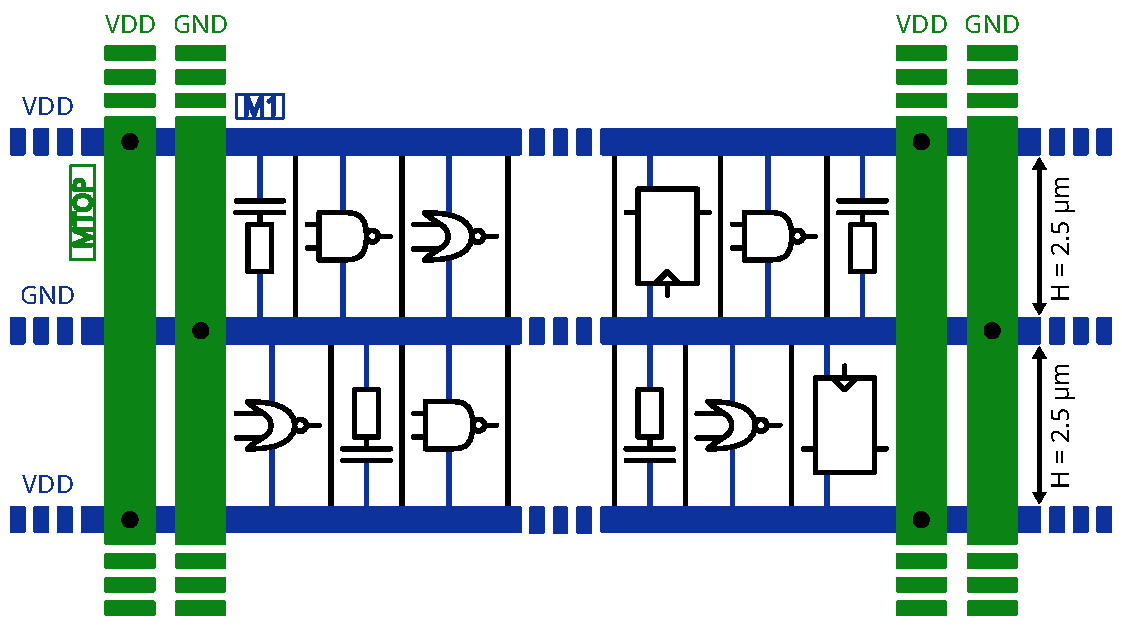
\includegraphics[width=0.49\textwidth]{./figures/psu_std_cell.pdf}
	\caption{A Standard-Cell Segment and its power delivery network.}
	\label{fig_alim_std}
\end{figure}


% !TeX spellcheck = en_US
% !TeX root = ./0_article.tex

\begin{figure}[h]
	\centering
	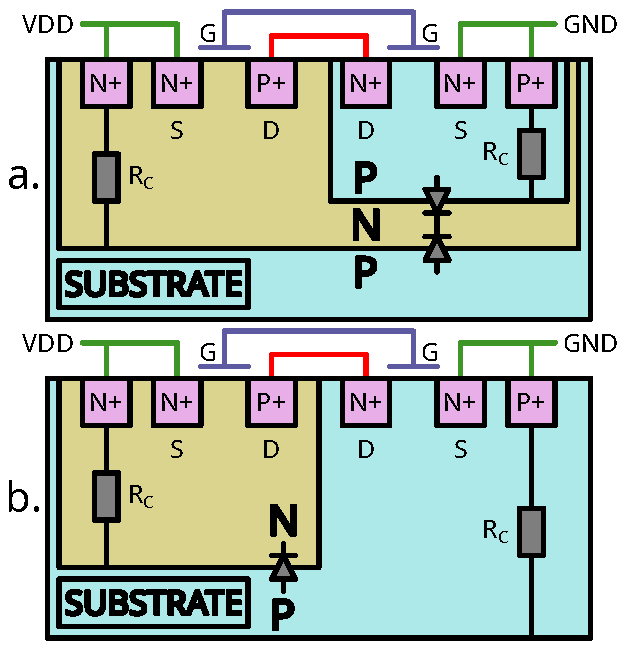
\includegraphics[width=0.35\textwidth]{./figures/substrate_2.pdf}
	\caption{Triple-well (a) and Dual-well (b) inverter cross-sectional view.}
	\label{fig_sub}
\end{figure}


% !TeX spellcheck = en_US
% !TeX root = ./0_article.tex

\begin{figure*}[ht]
	\centering
	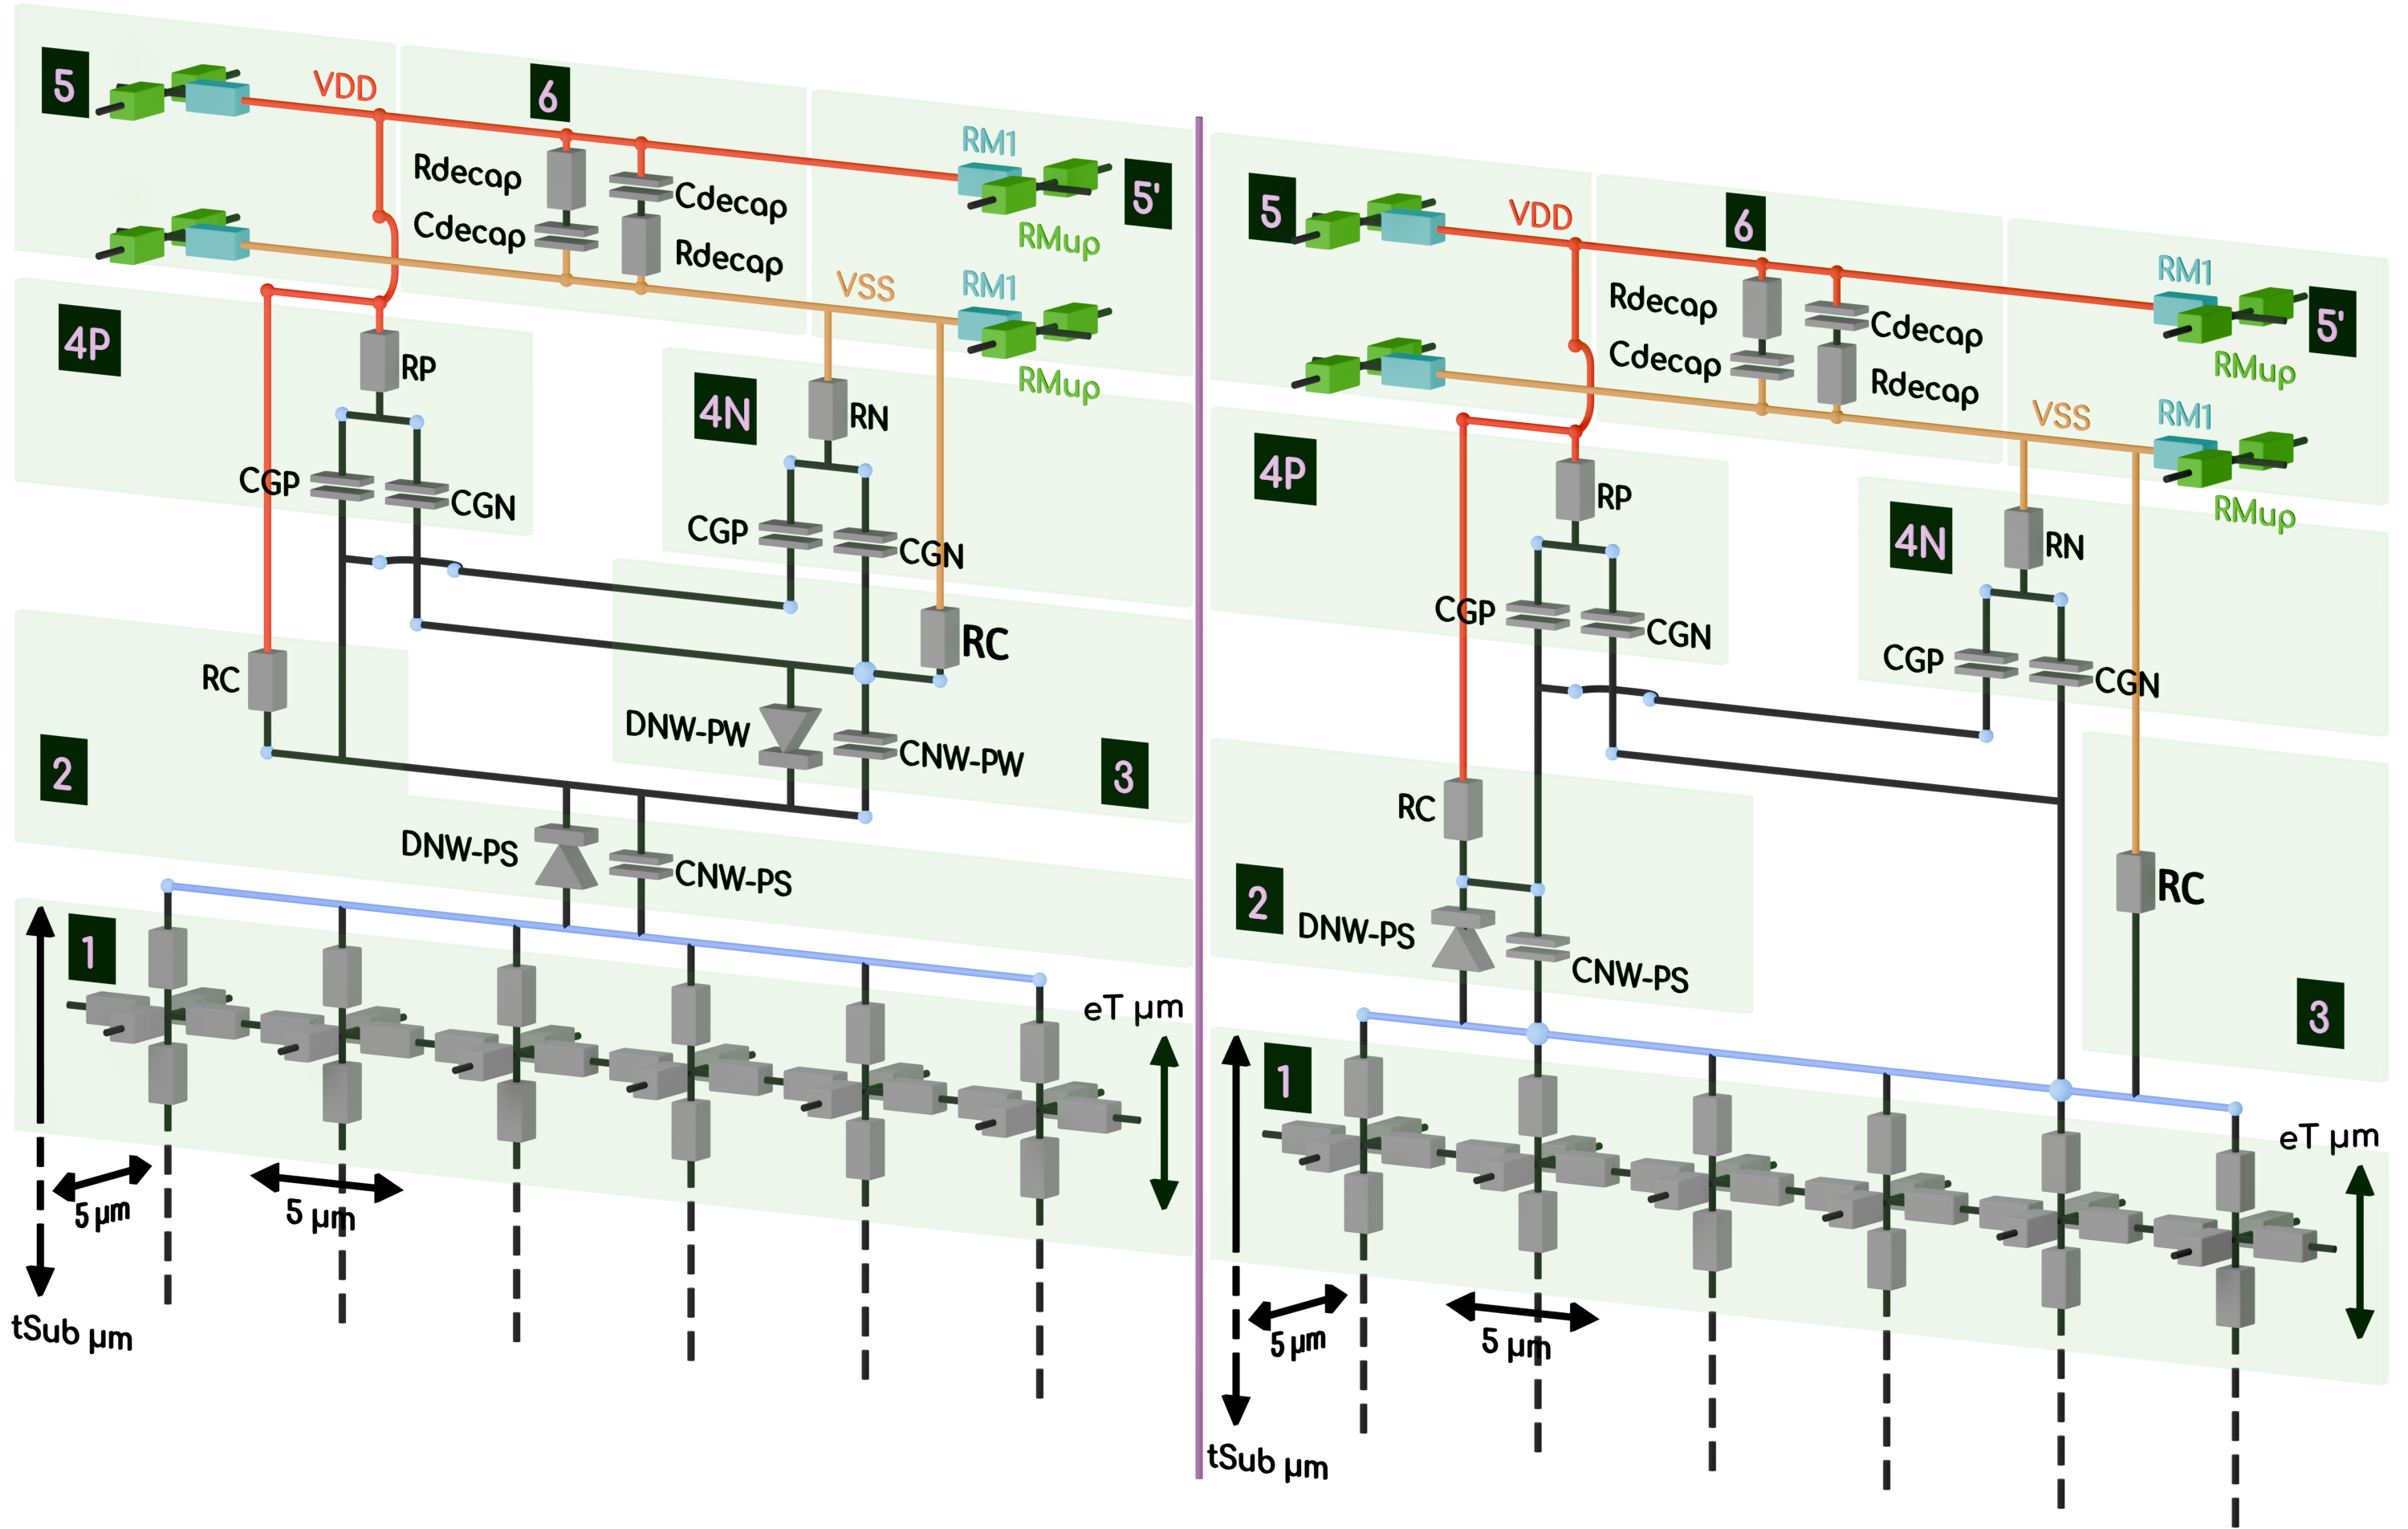
\includegraphics[width=0.95\textwidth]{./figures/dual+triple3.png}
	\caption{Triple well (left) and dual well (right) std cell \textcolor{red}{(PEUT ETRE FAIRE DES SOUS-FIGURES)}}
	\label{fig_triplewellstdcell}
\end{figure*}

